% ============================================================
% HSBI Beamer — ISLP Lecture Series — IMPROVED EDITION
% Chapter 13: Multiple Testing
% ============================================================
\documentclass[aspectratio=169,11pt]{beamer}
\usepackage[utf8]{inputenc}\usepackage[T1]{fontenc}\usepackage[english]{babel}
\usepackage{graphicx}\usepackage{booktabs}\usepackage{amsmath,amssymb,amsfonts}
\usepackage{mathtools}\usepackage{hyperref}\usepackage{xcolor}
\usepackage{verbatim}\usepackage{alltt}
\usepackage{tikz}\usetikzlibrary{calc,arrows.meta,positioning,shapes}
\usepackage{tcolorbox}\tcbuselibrary{skins}

\usetheme{Madrid}\usecolortheme{default}
\setbeamertemplate{navigation symbols}{}
\setbeamertemplate{footline}[frame number]
\setbeamertemplate{blocks}[rounded][shadow=false]
\setbeamertemplate{headline}{%
  \leavevmode\hbox{%
    \begin{beamercolorbox}[wd=\paperwidth,ht=2.2ex,dp=0.9ex]{section in head/foot}%
      {\fontsize{4.6}{5.2}\selectfont%
       \insertsectionnavigationhorizontal{\paperwidth}{}{\hskip0pt plus1filll}}%
    \end{beamercolorbox}}%
}
\setbeamerfont{section in head/foot}{size=\tiny}
\setbeamerfont{palette primary}{size=\tiny}
\setbeamerfont{palette tertiary}{size=\tiny}
\setbeamerfont{section in toc}{size=\footnotesize}

\usepackage{listings}
\definecolor{pyKw}{RGB}{0,0,180}\definecolor{pyStr}{RGB}{20,120,40}
\definecolor{pyCom}{RGB}{120,120,120}\definecolor{accent}{RGB}{38,70,140}
\lstdefinestyle{Pystyle}{language=Python,basicstyle=\ttfamily\footnotesize,
  keywordstyle=\color{pyKw}\bfseries,commentstyle=\color{pyCom}\itshape,
  stringstyle=\color{pyStr},showstringspaces=false,upquote=true,
  columns=fullflexible,breaklines=true,literate={~}{{$\sim$}}1}
\lstset{style=Pystyle}

\AtBeginSection[]{\begin{frame}{Outline}\footnotesize
  \tableofcontents[currentsection,sectionstyle=show/shaded,subsectionstyle=show/show/hide]
\end{frame}}

\newcommand{\islpsource}[1]{%
  \vfill\hfill{\tiny\itshape\color{gray}Source: #1 \textemdash{} ISLP, James et al.\ (2023).}\par
}

\newtcolorbox{takeaway}[1][Takeaway]{enhanced,colback=green!4,colframe=green!50!black,
  boxrule=0pt,leftrule=2.5pt,arc=2pt,fonttitle=\bfseries,title=#1,
  left=2mm,right=2mm,top=1mm,bottom=1mm}
\newtcolorbox{numexample}[1][Worked example]{enhanced,colback=orange!4,colframe=orange!70!black,
  boxrule=0pt,leftrule=2.5pt,arc=2pt,fonttitle=\bfseries,title=#1,
  left=2mm,right=2mm,top=1mm,bottom=1mm}
\newtcolorbox{readme}[1][How to read this]{enhanced,colback=blue!4,colframe=accent,
  boxrule=0pt,leftrule=2.5pt,arc=2pt,fonttitle=\bfseries,title=#1,
  left=2mm,right=2mm,top=1mm,bottom=1mm}

\title{An Introduction to Statistical Learning}
\subtitle{Chapter 13: Multiple Testing \textemdash{} Improved Edition}
\author{Prof.\ Dr.\ Christoph Weisser}\institute{HSBI}
\date{Summer Semester 2026}\graphicspath{{images/}}

\newtcolorbox{exercise}[1][Exercise]{enhanced, fontupper=\footnotesize, colback=purple!4, colframe=purple!55!black, boxrule=0pt, leftrule=2.5pt, arc=2pt, fonttitle=\bfseries, title=#1, left=2mm, right=2mm, top=1mm, bottom=1mm}
\newtcolorbox{solutionbox}[1][Solution]{enhanced, fontupper=\footnotesize, colback=teal!5, colframe=teal!55!black, boxrule=0pt, leftrule=2.5pt, arc=2pt, fonttitle=\bfseries, title=#1, left=2mm, right=2mm, top=1mm, bottom=1mm}
\newtcolorbox{longexercise}[1][Extended exercise (15 min)]{enhanced, fontupper=\footnotesize, colback=violet!6, colframe=violet!55!black, boxrule=0pt, leftrule=3pt, arc=2pt, fonttitle=\bfseries, title=#1, left=2mm, right=2mm, top=1mm, bottom=1mm}

% Reclaim ~2pt of body height (custom nav headline makes full slides tip over by ~1.83pt)
\addtobeamertemplate{frametitle}{}{\vspace{-2pt}}

\newtcolorbox{labnote}[1][Run this live in the lab notebook]{enhanced, fontupper=\footnotesize, colback=cyan!7, colframe=cyan!45!black, boxrule=0pt, leftrule=3pt, arc=2pt, fonttitle=\bfseries, title=#1, left=2mm, right=2mm, top=1mm, bottom=1mm}

\begin{document}
\begin{frame}[plain]\titlepage\end{frame}

\begin{frame}{The course at a glance}
  \footnotesize
  \begin{center}
  \begin{tabular}{@{}c r l@{}}
    & \textbf{Lecture} & \textbf{Topic}\\
    \midrule
     & 1 & Ch.\ 1 + 2 --- Introduction; what is statistical learning \\
     & 2 & Ch.\ 2 --- Accuracy, bias--variance, Bayes classifier, KNN \\
     & 3--4 & Ch.\ 3 --- Linear regression (estimation, inference, diagnostics) \\
     & 5--6 & Ch.\ 4 --- Classification (logistic, LDA/QDA, naive Bayes, ROC) \\
     & 7 & Ch.\ 5 --- Resampling (validation, CV, bootstrap) \\
     & 8 & Ch.\ 6 --- Model selection and regularisation (ridge, lasso) \\
     & 9 & Ch.\ 7 --- Moving beyond linearity (splines, GAMs) \\
     & 10 & Ch.\ 8 --- Tree-based methods (trees, forests, boosting) \\
     & 11 & Ch.\ 10 --- Deep learning (MLPs, CNNs, training) \\
    $\blacktriangleright$ & \textbf{12} & \textbf{Ch.\ 13 --- Multiple testing (FWER, FDR)} \\
  \end{tabular}
  \end{center}
  \vspace{2pt}
  {\scriptsize Twelve sessions of 180 minutes. $\blacktriangleright$ marks today's chapter. Short exercises every $\sim$20 min; extended exercises every $\sim$45 min; each chapter has a companion lab notebook.}
\end{frame}


\begin{frame}{Contents}\small\tableofcontents[hideallsubsections]\end{frame}

\begin{frame}{Notation in this chapter}
  \footnotesize
  \begin{center}
  \begin{tabular}{@{}ll@{}}
    \toprule
    \textbf{Symbol} & \textbf{Meaning} \\
    \midrule
    $m$ & number of hypotheses tested simultaneously \\
    $\alpha$ & per-test significance level; target FWER \\
    $H_{0j}$ & $j$-th null hypothesis in the family \\
    $p_j$, $p_{(j)}$ & $p$-value of test $j$; the $j$-th smallest (sorted) $p$-value \\
    $V$ & number of false positives (true nulls rejected) \\
    $R$ & total number of rejections, $R=V+S$ \\
    $S$ & number of true positives (false nulls rejected) \\
    FWER & family-wise error rate $\Pr(V\ge 1)$ \\
    FDR & false discovery rate $E\big[V/\max(R,1)\big]$ \\
    $q$ & target FDR level of Benjamini--Hochberg \\
    Power & $E[S]/m_1$, with $m_1$ the number of false nulls \\
    \bottomrule
  \end{tabular}
  \end{center}
\end{frame}

\begin{frame}{Sources and references}
  \begin{block}{Primary textbook}
    James et al.\ (2023). \emph{An Introduction to Statistical Learning,
    with Applications in Python.} Springer.
  \end{block}
\end{frame}

\begin{frame}{Learning objectives}
  By the end of this chapter you will be able to:
  \begin{itemize}
    \item \textbf{Explain} the multiple-testing problem and its
          consequences.
    \item \textbf{Apply} Bonferroni and Holm corrections to control
          family-wise error rate (FWER).
    \item \textbf{Apply} the Benjamini-Hochberg procedure to control
          false discovery rate (FDR).
    \item \textbf{Use} resampling-based $p$-values when the null
          distribution is hard to derive.
    \item \textbf{Avoid} the post-selection-inference and
          $p$-hacking pitfalls.
  \end{itemize}
\end{frame}


\begin{frame}{Roadmap of this chapter}
  \begin{takeaway}[Honest inference at scale]
    \begin{enumerate}
      \item The multiple-testing problem.
      \item FWER controls: Bonferroni, Holm.
      \item FDR control: Benjamini-Hochberg.
      \item Resampling-based $p$-values.
      \item Practical issues: $p$-hacking, post-selection inference.
    \end{enumerate}
  \end{takeaway}
\end{frame}

% ============================================================
\section{The Problem}
% ============================================================

\begin{frame}{Why naive testing fails at scale}
  Test $m$ hypotheses simultaneously, each at level $\alpha = 0.05$.
  \begin{numexample}[The arithmetic]
    \begin{itemize}
      \item Even if all $m$ nulls are true, we expect $0.05 m$ false
            rejections.
      \item Test $10\,000$ genes $\Rightarrow \sim 500$ false
            discoveries by chance.
      \item Naive thresholding fails dramatically.
    \end{itemize}
  \end{numexample}
\end{frame}

\begin{frame}{Why the family-wise error rate explodes}
  \begin{center}
    
\includegraphics[width=0.92\textwidth,height=0.58\textheight,keepaspectratio]{ch13_fwer.png}
  \end{center}
  \begin{takeaway}
    With $\alpha=0.05$ the chance of $\ge 1$ false positive passes $50\%$ by only $m=14$ tests and approaches certainty as $m$ grows.
  \end{takeaway}
\end{frame}

\begin{frame}{The classical hypothesis-test refresher}
  \begin{readme}
    \begin{itemize}
      \item $H_0$: null hypothesis. $H_1$: alternative.
      \item Type I error: reject $H_0$ when true.
      \item Type II error: fail to reject when false.
      \item $p$-value: probability under $H_0$ of a test statistic at
            least as extreme as observed.
      \item ``Reject $H_0$ if $p < \alpha$'' controls the per-test
            type-I error rate at $\alpha$.
    \end{itemize}
  \end{readme}
  \begin{takeaway}
    A $p$-value is computed \emph{assuming} $H_0$ is true; it is \textbf{not} the
    probability that $H_0$ is true, and a small $p$ is not proof of a large effect.
  \end{takeaway}
\end{frame}

\begin{frame}{The decision-table view}
  \begin{center}
  \begin{tabular}{l|cc|c}
    \toprule
            & Not rejected & Rejected & Total \\
    \midrule
    $H_0$ true   & $U$ & $V$ & $m_0$ \\
    $H_0$ false  & $T$ & $S$ & $m_1$ \\
    \midrule
    Total & $m - R$ & $R$ & $m$ \\
    \bottomrule
  \end{tabular}
  \end{center}
  \begin{readme}
    \begin{itemize}
      \item Family-wise error rate (FWER): $\Pr(V \ge 1)$.
      \item False discovery rate (FDR): $E[V/R \mid R > 0]\Pr(R > 0)$.
      \item Power: $E[S]/m_1$.
    \end{itemize}
  \end{readme}
\end{frame}

\begin{frame}{The four outcomes of a test decision}
  \begin{center}
  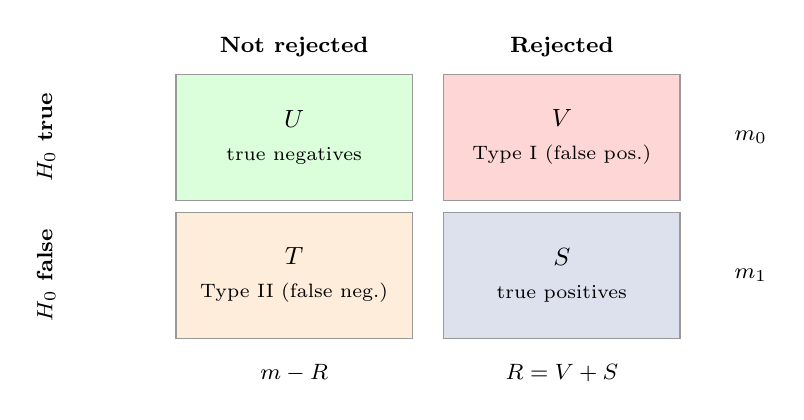
\begin{tikzpicture}[x=1cm,y=1cm,font=\small,
      cell/.style={minimum width=3cm,minimum height=1.6cm,draw=black!40,align=center},
      hd/.style={font=\footnotesize\bfseries}]
    \node[hd] at (1.6,1.15) {Not rejected};
    \node[hd] at (5.0,1.15) {Rejected};
    \node[hd,rotate=90] at (-1.55,0)     {$H_0$ true};
    \node[hd,rotate=90] at (-1.55,-1.75) {$H_0$ false};
    \node[cell,fill=green!14]  (U) at (1.6,0)     {$U$\\[1pt]\scriptsize true negatives};
    \node[cell,fill=red!16]    (V) at (5.0,0)     {$V$\\[1pt]\scriptsize Type I (false pos.)};
    \node[cell,fill=orange!14] (T) at (1.6,-1.75) {$T$\\[1pt]\scriptsize Type II (false neg.)};
    \node[cell,fill=accent!16] (S) at (5.0,-1.75) {$S$\\[1pt]\scriptsize true positives};
    \node[hd] at (7.4,0)     {$m_0$};
    \node[hd] at (7.4,-1.75) {$m_1$};
    \node[hd] at (1.6,-3.0)  {$m-R$};
    \node[hd] at (5.0,-3.0)  {$R=V+S$};
  \end{tikzpicture}
  \end{center}
  \begin{takeaway}
    \textbf{Type I errors} are the red cell $V$. The FWER $=\Pr(V\ge 1)$ guards against \emph{any} false positive; the FDR $=E[V/R]$ controls their \emph{expected fraction} among the $R$ rejections.
  \end{takeaway}
\end{frame}


% ------------------------------------------------------------
\begin{frame}{Exercise 13.1 --- The multiple-testing problem [Concept]}
\begin{exercise}
  \begin{enumerate}
    \item Define a Type I error and a Type II error in terms of $H_0$.
    \item Suppose $m$ hypotheses are tested independently, each at
          level $\alpha = 0.05$, and \emph{all} nulls are in fact
          true. Write the probability of making at least one false
          rejection (the FWER) as a function of $m$.
    \item Evaluate this probability for $m = 10$.
    \item Find the smallest $m$ for which the FWER reaches $0.5$.
  \end{enumerate}
\end{exercise}
\end{frame}

\begin{frame}{Solution --- Exercise 13.1 (1/2)}
\begin{solutionbox}
  \textbf{Method.} The FWER is easiest to reach through its complement: rather than
  count ``at least one false positive'' directly, find the single event ``no false
  positive at all'' and subtract from $1$.

  \medskip
  \textbf{Part 1 --- error types.}
  \begin{itemize}
    \item Type I (false positive): rejecting $H_0$ when it is true.
    \item Type II (false negative): failing to reject $H_0$ when it is
          false.
  \end{itemize}
  \medskip
  \textbf{Part 2 --- FWER formula.} One test avoids a false positive with
  probability $1 - \alpha$. Under independence the $m$ tests avoid it
  \emph{jointly} with probability $(1-\alpha)^m$ (independent probabilities
  multiply), so the complement is
  \[
    \mathrm{FWER}=\Pr(\text{at least one false positive})
    = 1 - (1 - \alpha)^m .
  \]
  \textit{Common mistake: adding the per-test rates to get $m\alpha$ --- that only
  approximates the FWER (the first-order term) and can exceed $1$.}
\end{solutionbox}
\end{frame}

\begin{frame}{Solution --- Exercise 13.1 (2/2)}
\begin{solutionbox}
  \textbf{Part 3 --- $m = 10$.}
  \[
    1 - (0.95)^{10} = 1 - 0.5987 = 0.4013 \approx 40\% .
  \]
  A $5\%$ per-test rate has ballooned to a $40\%$ chance of at least
  one spurious ``discovery''.
  \medskip
  \textbf{Part 4 --- FWER $= 0.5$.} Solve $1 - 0.95^m \ge 0.5$, i.e.
  $0.95^m \le 0.5$:
  \[
    m \ge \frac{\ln 0.5}{\ln 0.95}
        = \frac{-0.6931}{-0.05129} = 13.51 ,
  \]
  so $m = 14$ tests already give a better-than-even chance of a false
  positive. This is exactly why corrections are needed.

  \medskip
  \textit{Common mistake: dividing by $\ln 0.95$ without flipping the inequality.
  Since $\ln 0.95<0$, $\;0.95^m\le 0.5 \iff m\,\ln 0.95\le \ln 0.5 \iff
  m\ge \ln 0.5/\ln 0.95$ --- the sign flips at the last step.}
\end{solutionbox}
\end{frame}

% ============================================================
\section{FWER}
% ============================================================

\begin{frame}{Bonferroni: split the error budget equally}
  \begin{block}{Rule}
    \[
      \boxed{\;\text{Reject } H_{0j} \text{ if } p_j \le \alpha / m.\;}
    \]
  \end{block}
  \begin{readme}
    \begin{itemize}
      \item $m$: number of tests in the family; \ $\alpha$: target FWER (e.g.\ $0.05$).
      \item Divide the budget evenly: each test is judged at the stricter level
            $\alpha/m$.
      \item Equivalently, adjust each $p$-value to $\tilde p_j=\min(1,\,m\,p_j)$ and
            compare to $\alpha$.
    \end{itemize}
  \end{readme}
  \begin{takeaway}
    Controls FWER at $\alpha$ under \emph{any} dependence. Conservative: it throws away
    power, but is simple, popular, and a good starting point.
  \end{takeaway}
\end{frame}

\begin{frame}{Holm's step-down procedure (uniformly beats Bonferroni)}
  \begin{block}{Algorithm}
    \begin{enumerate}
      \item Order $p$-values
            $p_{(1)} \le p_{(2)} \le \cdots \le p_{(m)}$.
      \item Find the smallest $j$ with
            $p_{(j)} > \alpha/(m - j + 1)$.
      \item Reject all $H_{0(k)}$ for $k < j$.
    \end{enumerate}
  \end{block}
  \begin{readme}[Why it is more powerful]
    \begin{itemize}
      \item The thresholds \emph{grow} down the list:
            $\tfrac{\alpha}{m},\tfrac{\alpha}{m-1},\dots,\alpha$ --- the first equals
            Bonferroni, every later one is looser.
      \item ``Step-down'': start at the smallest $p$-value and walk down, stopping at
            the first test that fails; keep all larger $p$-values.
    \end{itemize}
  \end{readme}
  \begin{takeaway}
    Strictly more powerful than Bonferroni, yet still controls FWER at $\alpha$.
  \end{takeaway}
\end{frame}

\begin{frame}{Bonferroni vs.\ Holm on $15$ simulated $p$-values}
  \begin{center}
\includegraphics[width=0.88\textwidth,height=0.56\textheight,keepaspectratio]{ch13_x_holm_bonf.png}\end{center}
  \begin{takeaway}Bonferroni's flat bar $\alpha/m\approx 0.0033$ rejects $3$ hypotheses; Holm's rising thresholds $\alpha/(m-j+1)$ additionally catch $p_{(4)}=0.0041$, rejecting $4$ --- Holm always rejects at least as many as Bonferroni.\end{takeaway}
\end{frame}

\begin{frame}{Power loss with FWER control}
  \begin{center}
    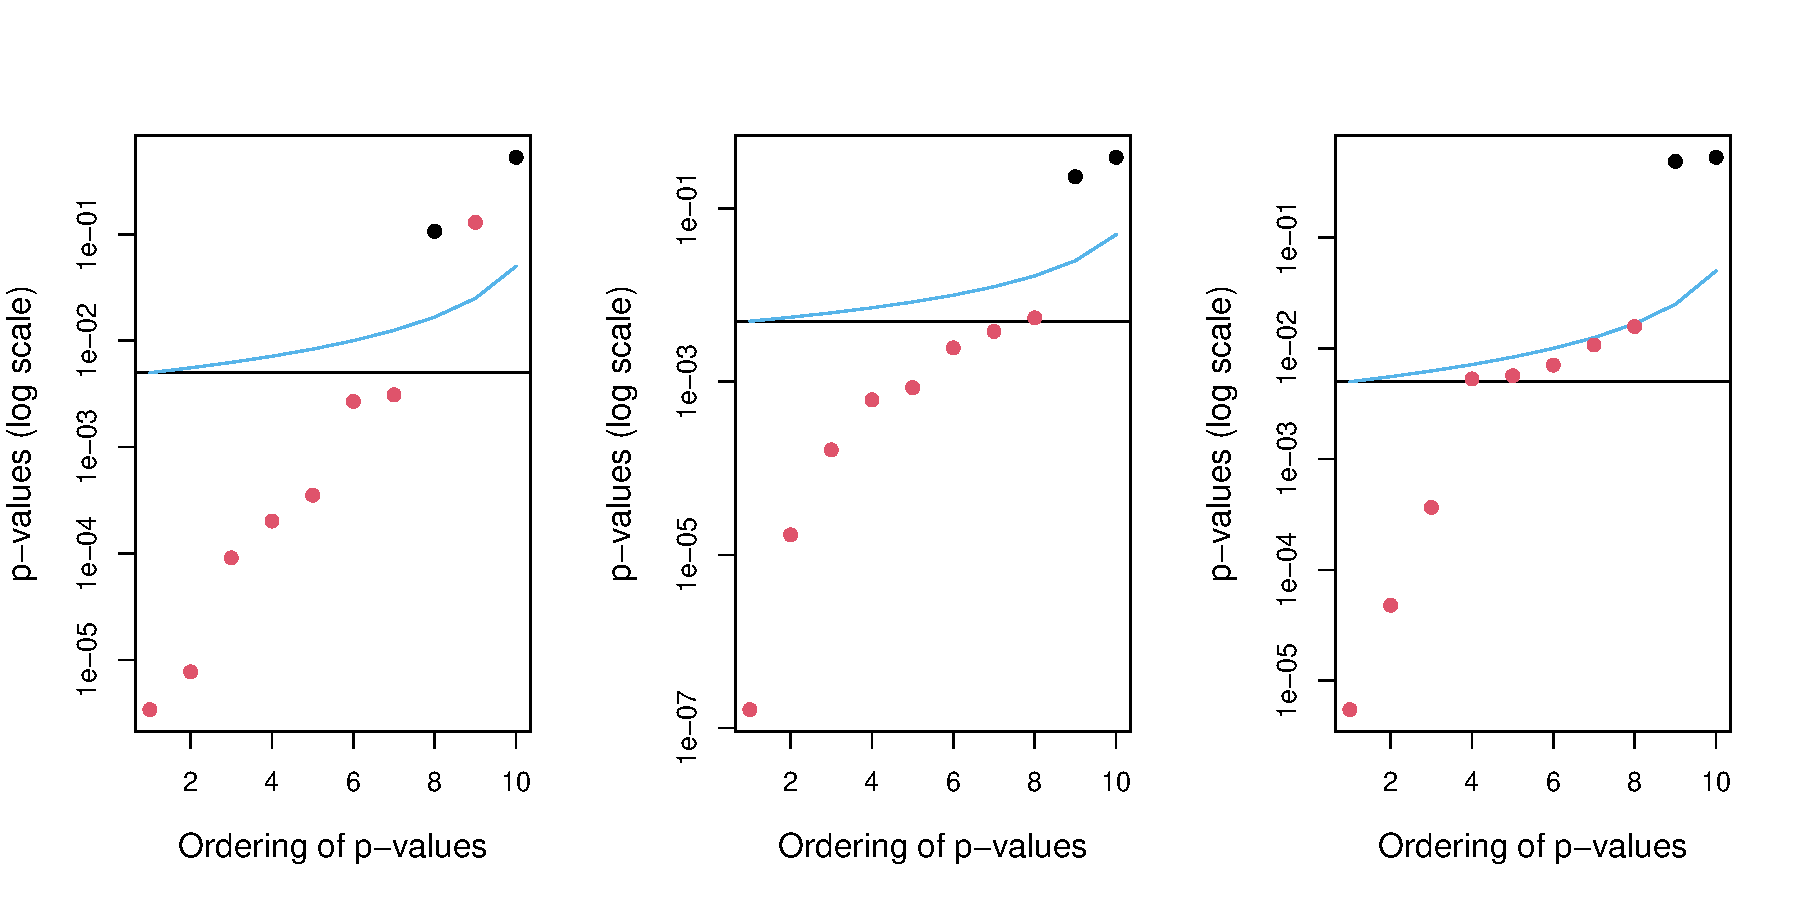
\includegraphics[width=0.85\textwidth,height=0.52\textheight,keepaspectratio]{13_3.pdf}
  \end{center}
  \begin{takeaway}
    Even Holm's procedure loses substantial power as $m$ grows: guarding against
    \emph{any} false positive forces tiny thresholds, so genuine effects slip through.
  \end{takeaway}
  \islpsource{Figure 13.3}
\end{frame}


% ------------------------------------------------------------
\begin{frame}{Exercise 13.2 --- Bonferroni correction [Math]}
\begin{exercise}
  You run $m = 6$ tests and obtain the sorted $p$-values
  \[
    p = (0.001,\; 0.008,\; 0.012,\; 0.030,\; 0.040,\; 0.600),
  \]
  and wish to control the FWER at $\alpha = 0.05$.
  \begin{enumerate}
    \item State the Bonferroni rejection threshold.
    \item Which hypotheses are rejected?
    \item Compute the Bonferroni-adjusted $p$-values
          $\tilde p_j = \min(1,\, m\, p_j)$ and confirm they give the
          same decisions.
  \end{enumerate}
\end{exercise}
\end{frame}

\begin{frame}{Solution --- Exercise 13.2}
\begin{solutionbox}
  \textbf{Step 1 --- threshold.}
  $\alpha / m = 0.05 / 6 = 0.00833$.

  \medskip
  \textbf{Step 2 --- reject if $p_j \le 0.00833$.}
  \[
    \begin{array}{l|cccccc}
      p_j        & 0.001 & 0.008 & 0.012 & 0.030 & 0.040 & 0.600 \\ \hline
      \le 0.00833? & \checkmark & \checkmark & \times & \times & \times & \times
    \end{array}
  \]
  Reject $H_1$ and $H_2$ only ($0.008 < 0.00833$; $0.012 > 0.00833$).

  \medskip
  \textbf{Step 3 --- adjusted $p$-values} $\tilde p_j = \min(1, 6 p_j)$:
  \[
    (0.006,\; 0.048,\; 0.072,\; 0.180,\; 0.240,\; 1.000).
  \]
  Rejecting when $\tilde p_j \le 0.05$ again flags exactly $H_1$
  ($0.006$) and $H_2$ ($0.048$). Two rejections.

  \medskip
  \textbf{Take-away.} Bonferroni is simple and valid under any
  dependence, but conservative --- here it misses $H_3$ at $p = 0.012$.
\end{solutionbox}
\end{frame}

\begin{frame}{Exercise 13.3 --- Holm's step-down procedure [Math]}
\begin{exercise}
  Using the same data as Exercise 13.2,
  \[
    p = (0.001,\; 0.008,\; 0.012,\; 0.030,\; 0.040,\; 0.600),
    \quad m = 6,\; \alpha = 0.05 ,
  \]
  apply Holm's step-down procedure. For each rank $j$ compare
  $p_{(j)}$ with $\alpha / (m - j + 1)$, stop at the first failure,
  and report the rejections. Compare with Bonferroni.
\end{exercise}
\end{frame}

\begin{frame}{Solution --- Exercise 13.3}
\begin{solutionbox}
  The $p$-values are already sorted. Compare each with its Holm
  threshold $\alpha / (m - j + 1)$:
  \[
    \begin{array}{c|c|c|c}
      j & p_{(j)} & \alpha/(m-j+1) & \text{decision} \\ \hline
      1 & 0.001 & 0.05/6 = 0.00833 & 0.001 \le 0.00833 \;\checkmark \\
      2 & 0.008 & 0.05/5 = 0.01000 & 0.008 \le 0.01000 \;\checkmark \\
      3 & 0.012 & 0.05/4 = 0.01250 & 0.012 \le 0.01250 \;\checkmark \\
      4 & 0.030 & 0.05/3 = 0.01667 & 0.030 > 0.01667 \;\times \\
    \end{array}
  \]
  The first failure is at $j = 4$. Holm rejects all hypotheses with
  rank $< 4$, i.e. $H_{(1)}, H_{(2)}, H_{(3)}$ --- \textbf{three}
  rejections.

  \medskip
  \textbf{Comparison.} Holm also rejects $H_{(3)}$ at $p = 0.012$,
  which Bonferroni missed. Holm is uniformly more powerful than
  Bonferroni while still controlling the FWER at $\alpha$, because its
  first threshold matches Bonferroni's but every later one is larger.
\end{solutionbox}
\end{frame}

% ============================================================
\section{FDR}
% ============================================================

\begin{frame}{The Benjamini-Hochberg (BH) procedure}
  \begin{block}{Algorithm (control FDR at level $q$)}
    \begin{enumerate}
      \item Order the $p$-values: $p_{(1)} \le \cdots \le p_{(m)}$.
      \item Find the largest $L$ such that $p_{(L)} \le L q / m$.
      \item Reject the $L$ smallest hypotheses.
    \end{enumerate}
  \end{block}
  \begin{readme}[Reading the threshold $Lq/m$]
    \begin{itemize}
      \item $q$: target FDR (e.g.\ $0.10$); \ $m$: number of tests; \ $L$: rank in the
            sorted list.
      \item The bar $Lq/m$ \emph{rises} with rank, unlike Bonferroni's flat $\alpha/m$.
      \item ``Step-up'': scan from the \emph{largest} $p$-value down; reject everything
            up to the first one that clears its bar.
    \end{itemize}
  \end{readme}
  \begin{takeaway}
    Under independence (or positive dependence), BH controls FDR at $q$.
  \end{takeaway}
\end{frame}

\begin{frame}{Visualising BH}
  \begin{center}
    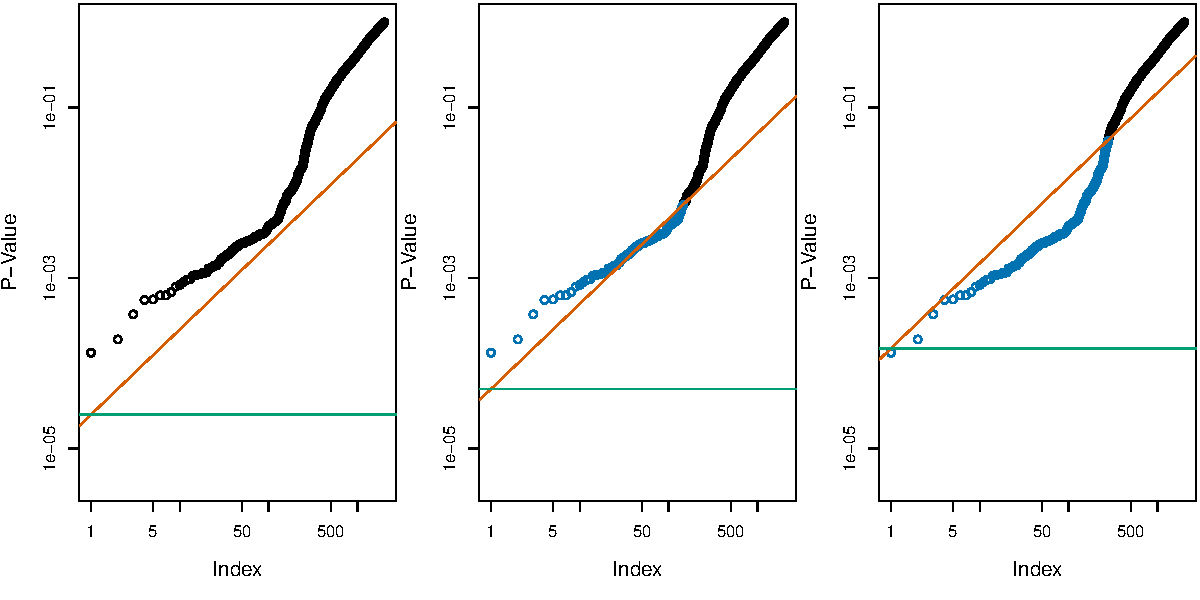
\includegraphics[width=0.85\textwidth,height=0.55\textheight,keepaspectratio]{13_6.pdf}
  \end{center}
  Sorted $p$-values vs.\ the line $L q / m$. Reject everything below
  the highest crossing.
  \islpsource{Figure 13.6}
\end{frame}

\begin{frame}{Benjamini-Hochberg as a staircase}
  \begin{center}
    
\includegraphics[width=0.92\textwidth,height=0.58\textheight,keepaspectratio]{ch13_bh.png}
  \end{center}
  \begin{takeaway}
    Compare each sorted $p_{(i)}$ with the line $(i/m)q$; take the \emph{largest} rank below it and reject everything up to there ($5$ of $30$ here at $q=0.10$).
  \end{takeaway}
\end{frame}

\begin{frame}{Three thresholds on the same six p-values}
  \begin{center}
    
\includegraphics[width=0.92\textwidth,height=0.52\textheight,keepaspectratio]{ch13_thresholds.png}
  \end{center}
  \begin{takeaway}
    A $p$-value is a candidate for rejection when it sits \emph{below} its method's
    curve. All three meet at rank $1$; then Bonferroni stays flat while Holm and BH
    rise --- so here they reject $2$, $3$ and $5$ hypotheses (Exercises 13.2/13.3/13.5).
  \end{takeaway}
\end{frame}

\begin{frame}{FDR vs.\ FWER: which to use?}
  \begin{readme}
    \begin{itemize}
      \item Use \textbf{FWER} when even one false discovery is
            unacceptable (drug-approval trials).
      \item Use \textbf{FDR} when an exploratory list of candidates
            is acceptable and false positives are tolerable in
            moderation (genomics, A/B testing).
      \item BH is much more powerful than Bonferroni when $m$ is
            large and a non-trivial fraction of nulls are false.
    \end{itemize}
  \end{readme}
\end{frame}


% ------------------------------------------------------------
\begin{frame}{Exercise 13.4 --- FDR vs.\ FWER [Concept]}
\begin{exercise}
  \begin{enumerate}
    \item Give the definitions of the FWER and the FDR in terms of the
          decision-table quantities $V$ (false rejections) and $R$
          (total rejections).
    \item Explain why controlling the FDR is generally less
          conservative (more powerful) than controlling the FWER.
    \item For each scenario, state whether FWER or FDR control is more
          appropriate and why: (i) a confirmatory phase-III drug
          trial; (ii) screening $20\,000$ genes for follow-up
          experiments.
  \end{enumerate}
\end{exercise}
\end{frame}

\begin{frame}{Solution --- Exercise 13.4 (1/2)}
\begin{solutionbox}
  \textbf{Part 1 --- definitions.}
  \[
    \text{FWER} = \Pr(V \ge 1),
    \qquad
    \text{FDR} = E\!\left[\frac{V}{R} \,\Big|\, R > 0\right]\Pr(R > 0).
  \]
  FWER is the probability of \emph{any} false positive; FDR is the
  \emph{expected proportion} of false positives among the rejections.

  \medskip
  \textbf{Part 2 --- why FDR is more powerful.} FWER guards against a
  single false positive anywhere, so its threshold must shrink with
  $m$ (roughly $\alpha/m$). FDR only requires the false positives to
  be a small \emph{fraction} of discoveries, so it tolerates a few
  errors when there are many true discoveries. This lets it use a
  larger, adaptive threshold and reject far more when many nulls are
  false.
\end{solutionbox}
\end{frame}

\begin{frame}{Solution --- Exercise 13.4 (2/2)}
\begin{solutionbox}
  \textbf{Part 3 --- scenarios.}
  \begin{itemize}
    \item[(i)] \textbf{FWER} (Bonferroni/Holm): a single false
          approval is unacceptable; the cost of any Type I error is
          very high.
    \item[(ii)] \textbf{FDR} (Benjamini-Hochberg): an exploratory
          candidate list is the goal; a modest fraction of false leads
          is acceptable and will be filtered by follow-up experiments.
          FWER here would be far too conservative and kill power.
  \end{itemize}
\end{solutionbox}
\end{frame}

\begin{frame}{Exercise 13.5 --- Benjamini-Hochberg procedure [Math]}
\begin{exercise}
  Using the same six $p$-values,
  \[
    p = (0.001,\; 0.008,\; 0.012,\; 0.030,\; 0.040,\; 0.600),
    \quad m = 6 ,
  \]
  apply the Benjamini-Hochberg (BH) procedure at FDR level
  $q = 0.05$.
  \begin{enumerate}
    \item For each rank $L$ compute the BH threshold $L q / m$.
    \item Find the largest $L$ with $p_{(L)} \le L q / m$.
    \item State the rejections and compare with Bonferroni and Holm.
  \end{enumerate}
\end{exercise}
\end{frame}

\begin{frame}{Solution --- Exercise 13.5 (1/2)}
\begin{solutionbox}
  \textbf{Steps 1--2 --- compare each $p_{(L)}$ with $L q / m$,}
  where $q/m = 0.05/6 = 0.00833$:
  \[
    \begin{array}{c|c|c|c}
      L & p_{(L)} & Lq/m & p_{(L)} \le Lq/m ? \\ \hline
      1 & 0.001 & 0.00833 & \checkmark \\
      2 & 0.008 & 0.01667 & \checkmark \\
      3 & 0.012 & 0.02500 & \checkmark \\
      4 & 0.030 & 0.03333 & \checkmark \\
      5 & 0.040 & 0.04167 & \checkmark \\
      6 & 0.600 & 0.05000 & \times \\
    \end{array}
  \]
  The largest $L$ satisfying the condition is $L = 5$.
\end{solutionbox}
\end{frame}

\begin{frame}{Solution --- Exercise 13.5 (2/2)}
\begin{solutionbox}
  \textbf{Step 3 --- reject.} BH rejects the $5$ smallest hypotheses
  $H_{(1)}, \ldots, H_{(5)}$ (everything except $p = 0.600$).

  \medskip
  \textbf{Comparison on identical data.}
  \[
    \text{Bonferroni: 2} \;\;<\;\; \text{Holm: 3}
    \;\;<\;\; \text{BH: 5 rejections.}
  \]
  Controlling the FDR yields many more discoveries than controlling
  the FWER --- at the price of allowing a small expected fraction
  ($\le q$) of them to be false. Note BH is a \emph{step-up} rule: even
  though $p_{(4)} = 0.030$ and $p_{(5)} = 0.040$ individually clear
  their thresholds here, BH would reject them via the largest passing
  $L$ regardless of any earlier borderline case.
\end{solutionbox}
\end{frame}

% ------------------------------------------------------------
% EXTENDED (INTEGRATIVE) EXERCISE 13.1 --- Bonferroni / Holm / BH full workflow
\begin{frame}{Extended Exercise 13.1 --- Full workflow on ten p-values [Math]}
\begin{longexercise}
  Ten hypotheses give the sorted $p$-values
  \[
    p=(0.0008,\,0.0041,\,0.0060,\,0.0100,\,0.0180,\,0.0290,\,0.0850,\,0.150,\,0.240,\,0.790),
  \]
  with $m=10$. Control the FWER at $\alpha=0.05$ (Bonferroni, Holm) and the FDR at
  $q=0.10$ (Benjamini--Hochberg).
  \begin{enumerate}
    \item List the rejections under \textbf{Bonferroni}, \textbf{Holm} and \textbf{BH}.
    \item Verify the ordering $R_{\text{Bonf}}\le R_{\text{Holm}}\le R_{\text{BH}}$.
    \item State the guaranteed FWER bound, and comment on what the FDR guarantee buys.
  \end{enumerate}
\end{longexercise}
\end{frame}

\begin{frame}{Solution --- Extended Exercise 13.1 (1/3)}
\begin{solutionbox}[Bonferroni and Holm (FWER $\le 0.05$)]
  \textbf{Bonferroni:} reject if $p_j\le\alpha/m=0.005$. Only $p_{(1)}=0.0008$ and
  $p_{(2)}=0.0041$ qualify $\Rightarrow$ \textbf{2 rejections}.
  \medskip
  \textbf{Holm:} compare $p_{(j)}$ with $\alpha/(m-j+1)$, stopping at the first failure:
  \[
    \begin{array}{c|c|c|c}
      j & p_{(j)} & \alpha/(m-j+1) & \\ \hline
      1 & 0.0008 & 0.05/10=0.00500 & \checkmark\\
      2 & 0.0041 & 0.05/9=0.00556 & \checkmark\\
      3 & 0.0060 & 0.05/8=0.00625 & \checkmark\\
      4 & 0.0100 & 0.05/7=0.00714 & \times\ \text{stop}
    \end{array}
  \]
  Holm rejects ranks $1$--$3$ $\Rightarrow$ \textbf{3 rejections}.
\end{solutionbox}
\end{frame}

\begin{frame}{Solution --- Extended Exercise 13.1 (2/3)}
\begin{solutionbox}[Benjamini--Hochberg (FDR $\le 0.10$)]
  Compare each $p_{(L)}$ with $Lq/m=0.01L$ and take the \emph{largest} passing $L$:
  \[
    \begin{array}{c|c|c|c}
      L & p_{(L)} & Lq/m & \\ \hline
      5 & 0.0180 & 0.050 & \checkmark\\
      6 & 0.0290 & 0.060 & \checkmark\ \leftarrow \text{largest}\\
      7 & 0.0850 & 0.070 & \times\\
      8 & 0.150  & 0.080 & \times
    \end{array}
  \]
  (Ranks $1$--$4$ pass too.) The largest $L$ with $p_{(L)}\le Lq/m$ is $L=6$, so BH
  rejects the six smallest $\Rightarrow$ \textbf{6 rejections} --- including
  $p_{(6)}=0.029$ and ranks $4,5$ that the FWER rules missed.
\end{solutionbox}
\end{frame}

\begin{frame}{Solution --- Extended Exercise 13.1 (3/3)}
\begin{solutionbox}[Comparison and error guarantees]
  \[
    \underbrace{2}_{\text{Bonferroni}}\ \le\
    \underbrace{3}_{\text{Holm}}\ \le\
    \underbrace{6}_{\text{BH}} .
  \]
  \textbf{FWER bound.} Bonferroni and Holm both guarantee
  $\mathrm{FWER}=\Pr(V\ge1)\le\alpha=0.05$ under \emph{any} dependence: the chance of
  \emph{even one} false rejection is at most $5\%$.
  \medskip
  \textbf{What FDR buys.} BH instead guarantees
  $\mathrm{FDR}=E[V/R]\le q\,m_0/m\le 0.10$. Among its $6$ discoveries, at most an
  \emph{expected} $10\%$ ($\lesssim1$ here) are false. Tolerating a small false
  \emph{fraction} rather than \emph{any} false positive is exactly why BH rejects more.
\end{solutionbox}
\end{frame}

% ============================================================
\section{Resampling}
% ============================================================

\begin{frame}{Resampling-based $p$-values}
  When the test statistic's null distribution is hard to derive:
  \begin{readme}
    \begin{itemize}
      \item \textbf{Permutation}: shuffle the response many times to
            get a null distribution.
      \item \textbf{Bootstrap (under $H_0$)}: resample under a
            constraint that enforces the null.
      \item Empirical $p$-values are then thresholded by Bonferroni /
            Holm / BH as before.
    \end{itemize}
  \end{readme}
  \begin{takeaway}
    Empirical $p$-value $=\dfrac{1+\#\{\text{resampled statistics}\ge\text{observed}\}}{1+B}$
    over $B$ resamples --- no parametric null needed. The ``$+1$'' keeps it strictly
    positive.
  \end{takeaway}
\end{frame}

\begin{frame}{Resampling-based FDR}
  \begin{takeaway}[Storey's $q$-value]
    Estimate the proportion of true nulls $\hat\pi_0$ from the
    $p$-value distribution. Calibrate FDR more accurately than BH.
    Especially relevant when many nulls are false.
  \end{takeaway}
  \begin{readme}[How $\hat\pi_0$ is read off]
    True nulls give $p$-values that are $\sim U(0,1)$, so the histogram is \emph{flat}
    away from $0$; the height of that flat part estimates $\hat\pi_0$. BH implicitly
    assumes $\hat\pi_0=1$; plugging in the smaller true value makes FDR control less
    conservative and recovers more discoveries.
  \end{readme}
\end{frame}

\begin{frame}{The distribution of $p$-values under many tests}
  \begin{center}
    
\includegraphics[width=0.92\textwidth,height=0.58\textheight,keepaspectratio]{ch13_pval_hist.png}
  \end{center}
  \begin{takeaway}
    True nulls give $p$-values that are $\sim U(0,1)$ (the flat bulk), while true effects pile up near $0$. Storey's method reads $\hat\pi_0$ off the height of that flat part to calibrate the FDR.
  \end{takeaway}
\end{frame}


% ============================================================
\section{Practice}
% ============================================================

\begin{frame}{$p$-hacking and selection bias}
  \begin{alertblock}{Don't}
    \begin{itemize}
      \item Report only the most-significant subset of tests.
      \item Test thousands of hypotheses and call the smallest
            $p$-value ``significant''.
    \end{itemize}
  \end{alertblock}
  \begin{takeaway}
    Multiple-testing correction must include \emph{every} test you
    ran, not only the ones you report. Pre-register hypotheses where
    possible; out-of-sample replication is the gold standard.
  \end{takeaway}
\end{frame}

\begin{frame}{Post-selection inference}
  After variable selection (lasso, stepwise) standard $p$-values are
  invalid.
  \begin{takeaway}
    The bias: the \emph{same data} both \emph{chose} the hypothesis and \emph{tested}
    it, so the reported $p$-values are optimistically small. Valid inference must
    account for the selection step.
  \end{takeaway}
  \begin{readme}[Modern methods]
    \begin{itemize}
      \item Sample splitting / data-carving.
      \item Selective inference (Lee, Sun, Sun, Taylor).
      \item Knockoffs (Barber, Cand\`es).
    \end{itemize}
  \end{readme}
\end{frame}

% ------------------------------------------------------------
% EXTENDED (INTEGRATIVE) EXERCISE 13.2 --- FWER vs FDR design decision
\begin{frame}{Extended Exercise 13.2 --- FWER or FDR? A design decision [Integrative]}
\begin{longexercise}
  For each study, choose an error criterion and justify it, using the naive expected
  number of false discoveries $E[V]=m_0\,\alpha$ (all-null worst case $m_0=m$) and the
  power consequences.
  \begin{enumerate}
    \item \textbf{Scenario A --- confirmatory phase-III trial:} $m=4$ co-primary
          endpoints; one false ``significant'' endpoint could license an ineffective drug.
    \item \textbf{Scenario B --- exploratory screen:} $m=20\,000$ genes tested for
          follow-up; a shortlist with a few false leads is acceptable.
    \item Contrast the statistical power the two criteria leave on the table.
  \end{enumerate}
\end{longexercise}
\end{frame}

\begin{frame}{Solution --- Extended Exercise 13.2 (1/3)}
\begin{solutionbox}[Scenario A --- confirmatory trial: control FWER]
  With $m=4$ tests at $\alpha=0.05$, naive testing expects
  \[
    E[V]=m_0\alpha=4(0.05)=0.20\ \text{false positives},\qquad
    \mathrm{FWER}=1-0.95^4=0.185 .
  \]
  A $\sim$$19\%$ chance of \emph{any} false endpoint is unacceptable when the decision is
  regulatory and irreversible. \textbf{Choose FWER control} (Bonferroni threshold
  $\alpha/m=0.0125$, or Holm). One false positive is the outcome we must not allow, so we
  pay the power cost gladly --- with only $m=4$ tests that cost is tiny.
\end{solutionbox}
\end{frame}

\begin{frame}{Solution --- Extended Exercise 13.2 (2/3)}
\begin{solutionbox}[Scenario B --- exploratory screen: control FDR]
  With $m=20\,000$ and (worst case) $m_0\approx20\,000$, naive testing expects
  \[
    E[V]=m_0\alpha=20\,000(0.05)=1000\ \text{false discoveries!}
  \]
  Bonferroni would shrink the threshold to $\alpha/m=2.5\times10^{-6}$, cutting $E[V]$ to
  $\approx0.05$ but \textbf{destroying power} for realistic effect sizes. \textbf{Choose
  FDR control} (BH at $q=0.10$): accept that an expected $\le 10\%$ of the shortlist is
  false in exchange for detecting far more true signals --- the false leads are removed by
  follow-up experiments.
\end{solutionbox}
\end{frame}

\begin{frame}{Solution --- Extended Exercise 13.2 (3/3)}
\begin{solutionbox}[The power trade-off]
  \begin{center}\footnotesize
  \begin{tabular}{lll}
    \toprule
     & Confirmatory ($m=4$) & Exploratory ($m=20\,000$) \\
    \midrule
    Criterion       & FWER (Bonferroni/Holm) & FDR (BH) \\
    Threshold shape & $\alpha/m$ (fixed, tiny) & adaptive $Lq/m$ \\
    Naive $E[V]$    & $0.20$ & $1000$ \\
    Priority        & no false positive & many true findings \\
    \bottomrule
  \end{tabular}
  \end{center}
  \textbf{Trade-off.} The FWER threshold shrinks like $\alpha/m$, so power collapses as
  $m$ grows --- fine for a handful of endpoints, ruinous for $20\,000$ genes. FDR asks
  only that false positives be a small \emph{fraction} of discoveries, so its adaptive
  threshold keeps power high at scale. \textbf{Rule of thumb:} match the criterion to the
  cost of a single false positive.
\end{solutionbox}
\end{frame}

% ============================================================
\section{Python Lab}

\begin{frame}{Python lab --- run it live in the notebook}
  \begin{labnote}[Companion notebook: \texttt{chapter\_13\_lab.ipynb}]
    The code in this section is meant to be \textbf{demonstrated live}. Open the companion Jupyter notebook and run it cell by cell:
    \begin{itemize}
      \item simulating $m=1000$ tests with a fraction of true effects;
      \item comparing Bonferroni, Holm and Benjamini--Hochberg;
      \item visualising the BH threshold line and a permutation test.
    \end{itemize}
    Data loads via the \texttt{ISLP} package or the bundled CSV files; the notebook ends with hands-on exercises.
  \end{labnote}
\end{frame}


% ============================================================

\begin{frame}[fragile]{Bonferroni, Holm, BH in statsmodels}
  \begin{lstlisting}
from statsmodels.stats.multitest import multipletests  # corrections
import numpy as np                                     # arrays

p = np.array([1e-6, 0.01, 0.04, 0.05, 0.30, 0.45, 0.80])  # raw p-values

for method in ["bonferroni", "holm", "fdr_bh"]:  # FWER, FWER, FDR control
    rej, p_corr, *_ = multipletests(p, alpha=0.05, method=method)  # adjust
    print(f"{method:12s}", rej)                   # rejection flags (bool)
    print(f"{'p_adj':12s}", np.round(p_corr, 4))  # adjusted p-values
  \end{lstlisting}
\end{frame}

% ------------------------------------------------------------
% EXTENDED (INTEGRATIVE) EXERCISE 13.3 --- simulate FDR and power
\begin{frame}{Extended Exercise 13.3 --- Simulating FDR and power [Python]}
\begin{longexercise}
  Simulate $m=1000$ one-sided $z$-tests of which $m_1=100$ have a true effect
  (mean shift $\mu=3$); the other $900$ are null. Over many repeats, apply
  Benjamini--Hochberg at $q=0.10$ and Bonferroni at $\alpha=0.05$, and estimate the
  \emph{realised} FDR ($V/R$) and power ($S/m_1$) of each.
  \begin{enumerate}
    \item Write the simulation and run $\sim2000$ repeats.
    \item Report the realised FDR and power for BH and for Bonferroni.
    \item Check BH against its theoretical bound $q\,m_0/m$, and comment on the power gap.
  \end{enumerate}
\end{longexercise}
\end{frame}

\begin{frame}[fragile]{Solution --- Extended Exercise 13.3 (1/3)}
\begin{solutionbox}[Code: setup and the BH rule]
\begin{lstlisting}
import numpy as np                 # arrays and random numbers
from scipy import stats            # normal cdf for p-values
rng = np.random.default_rng(0)     # seeded generator: reproducible
m, m1, mu = 1000, 100, 3.0         # 100 true effects, mean shift mu
q, alpha  = 0.10, 0.05             # FDR target q, FWER target alpha
truth = np.arange(m) < m1          # first m1 tests are non-null

def bh_reject(p, q):               # Benjamini-Hochberg step-up
    order = np.argsort(p); ps = p[order]      # sort p-values ascending
    thr = (np.arange(1, m + 1) / m) * q       # BH line: (j/m) * q
    hit = np.where(ps <= thr)[0]              # ranks below the line
    rej = np.zeros(m, bool)                   # start: reject nothing
    if len(hit): rej[order[:hit.max() + 1]] = True  # up to largest hit
    return rej                                # boolean rejection mask
\end{lstlisting}
\end{solutionbox}
\end{frame}

\begin{frame}[fragile]{Solution --- Extended Exercise 13.3 (2/3)}
\begin{solutionbox}[Code: simulate FDR and power]
\begin{lstlisting}[basicstyle=\ttfamily\scriptsize]
def simulate(method, reps=2000):                   # average FDR / power over reps
    fdr = pw = 0.0                                 # running totals
    for _ in range(reps):
        z = rng.normal(0, 1, m); z[:m1] = rng.normal(mu, 1, m1)  # effects: mean mu
        p = 1 - stats.norm.cdf(z)                  # one-sided p-values
        rej = bh_reject(p, q) if method == "bh" else (p <= alpha / m)  # BH or Bonf.
        V = (rej & ~truth).sum(); S = (rej & truth).sum(); R = rej.sum()  # V, S, R
        fdr += V / max(R, 1); pw += S / m1         # realised FDP and power
    return fdr / reps, pw / reps                   # averages over the repeats

for meth in ["bh", "bonferroni"]:                  # compare both procedures
    f, p = simulate(meth)                          # run the experiment
    print("%-11s FDR=%.3f power=%.3f" % (meth, f, p))  # summary line
\end{lstlisting}
\end{solutionbox}
\end{frame}

\begin{frame}{Solution --- Extended Exercise 13.3 (3/3)}
\begin{solutionbox}[Expected numbers and interpretation]
  \textbf{Typical printout.}
  \begin{center}\ttfamily\footnotesize
  bh\quad FDR=0.090\quad power=0.723\\[2pt]
  bonferroni\quad FDR=0.002\quad power=0.186
  \end{center}
  \begin{itemize}
    \item \textbf{BH} holds the realised FDR at $0.090$ --- essentially its theoretical
          ceiling $q\,m_0/m=0.10\times900/1000=0.09$ --- while recovering about
          \textbf{72\%} of the true effects.
    \item \textbf{Bonferroni} is far stricter: realised FDR $\approx0.002$, but power
          collapses to about \textbf{19\%} --- it misses four-fifths of the signals.
    \item \textbf{Lesson:} at $m=1000$, FDR control detects roughly \emph{four times} as
          many true effects as FWER control, for a small, bounded false fraction.
  \end{itemize}
\end{solutionbox}
\end{frame}

% ============================================================
\section{Summary}
% ============================================================

\begin{frame}{Chapter 13 in one slide}
  \begin{block}{What we accomplished}
    Honest inference when many hypotheses are tested at once.
  \end{block}
  \begin{itemize}
    \item Set up the multiple-testing problem.
    \item Family-wise error rate (FWER): Bonferroni and Holm.
    \item False discovery rate (FDR): Benjamini-Hochberg.
    \item Resampling-based $p$-values and Storey's $q$-values.
    \item Pitfalls of post-selection inference and $p$-hacking.
  \end{itemize}
\end{frame}

\begin{frame}{Key formulas at a glance}
  \footnotesize
  \begin{description}
    \item[FWER] $\mathrm{FWER}=\Pr(V\ge 1)=1-(1-\alpha)^m$ \ (independent tests).
    \item[Bonferroni] reject $H_{0j}$ if $p_j\le \alpha/m$ \ (controls FWER).
    \item[Holm] reject while $p_{(j)}\le \dfrac{\alpha}{m-j+1}$, stepping down from the smallest.
    \item[FDR] $\mathrm{FDR}=E\!\left[\dfrac{V}{\max(R,1)}\right]$ \ (expected false-discovery proportion).
    \item[Benjamini--Hochberg] reject the $L$ smallest, where $L=\max\{j: p_{(j)}\le \tfrac{j}{m}q\}$.
    \item[Power] $\mathrm{Power}=E[S]/m_1$.
  \end{description}
\end{frame}

\begin{frame}{Vocabulary checklist}
  \footnotesize
  \begin{tabular}{ll}
    \toprule
    \textbf{Term} & \textbf{Meaning} \\
    \midrule
    Type I error & Reject $H_0$ when true \\
    Type II error & Fail to reject when false \\
    FWER $= \Pr(V \ge 1)$ & Family-wise error rate \\
    FDR $= E[V/R]$ & False discovery rate \\
    Bonferroni / Holm & FWER controls \\
    BH procedure & Step-up FDR control \\
    Storey's $q$-value & FDR-calibrated $p$-value \\
    Permutation test & Null distribution by relabelling \\
    Knockoffs & Modern FDR control with covariate engineering \\
    \bottomrule
  \end{tabular}
\end{frame}

\begin{frame}{Decision rules of thumb}
  \begin{itemize}
    \item Always specify the family of tests \emph{before} looking at
          the data.
    \item Confirmatory / regulated $\Rightarrow$ FWER (Bonferroni or
          Holm).
    \item Exploratory / discovery $\Rightarrow$ BH on FDR.
    \item Report both raw and adjusted $p$-values.
    \item Replicate findings on an independent sample whenever
          possible.
    \item For valid post-selection inference: sample-splitting,
          selective inference, knockoffs.
  \end{itemize}
\end{frame}

\begin{frame}{Common pitfalls}
  \begin{alertblock}{Don't}
    \begin{enumerate}
      \item Test thousands of hypotheses and report only the
            ``significant'' ones.
      \item Use BH when tests are strongly negatively dependent.
      \item Confuse FWER and FDR --- they answer different questions.
      \item Apply post-hoc multiple-testing fixes after looking at
            the data.
      \item Use uncorrected $p$-values from stepwise / lasso.
      \item Treat a $p$-value as a probability that $H_0$ is true.
    \end{enumerate}
  \end{alertblock}
\end{frame}

\begin{frame}{Course-wide summary}
  \begin{block}{The conceptual arc}
    \begin{enumerate}
      \item Vocabulary and bias-variance (Ch.~1--2).
      \item Linear baselines and how to evaluate them (Ch.~3--5).
      \item Regularisation and dimension reduction (Ch.~6).
      \item Adding flexibility: splines, GAMs, trees, SVMs, deep nets
            (Ch.~7--10).
      \item Special responses: censored times, no response
            (Ch.~11--12).
      \item Honest inference at scale (Ch.~13).
    \end{enumerate}
  \end{block}
\end{frame}

\begin{frame}{Closing thoughts}
  \begin{takeaway}[The four habits of an effective statistical learner]
    \begin{enumerate}
      \item Always plot the data.
      \item Always validate on data you didn't train on.
      \item Always interpret what the model says about the world.
      \item Always check assumptions and limitations before claiming
            results.
    \end{enumerate}
  \end{takeaway}
  Thank you for taking this course. Good luck applying statistical
  learning to your own data!
\end{frame}

\end{document}
